\documentclass[11pt,a4paper]{scrartcl}

% ------------------------------------------------------------

% Packages
\usepackage{mathtools}
\usepackage{amssymb}
\usepackage{tikz-qtree}
\usepackage[hidelinks]{hyperref}
\usepackage{titlesec}
\usepackage{tocloft}
\usepackage[cm]{fullpage}
\usepackage{csquotes}
\usepackage{wrapfig}
\usepackage{listings}
\usepackage{xcolor}
\usepackage{makeidx}
\usepackage{ulem}

\usepackage{graphicx}
\graphicspath{{images/}}

\usepackage{parskip}
\setlength{\parindent}{0pt}

%% Packages used for symbols and signs like (c), €
\usepackage{textcomp,units}
\usepackage{enumerate}

%% Package used for nice block text
\usepackage{microtype}

\usepackage{ellipsis}
\usepackage{fixltx2e}
\usepackage{booktabs}

%% Package used for correction of wrong display 'Marginalien'
\usepackage{mparhack}

%% Package used for nicer tables
\usepackage{longtable}

%% Packages used to break long urls
\usepackage{url}
\usepackage{etoolbox}
\appto\UrlBreaks{\do\a\do\b\do\c\do\d\do\e\do\f\do\g\do\h\do\i\do\j
\do\k\do\l\do\m\do\n\do\o\do\p\do\q\do\r\do\s\do\t\do\u\do\v\do\w
\do\x\do\y\do\z}

%% Package used for German descriptions
\usepackage[ansinew]{inputenc}
\usepackage[ngerman]{babel}
\addto\captionsngerman{ 
    \renewcommand{\figurename}{Abbildung} 
    \renewcommand{\tablename}{Tabelle}
    \renewcommand{\abstractname}{Kurzfassung}
    %\renewcommand{\nomname}{Abkürzungen}
    \renewcommand{\lstlistingname}{Snippet}
    \renewcommand{\lstlistlistingname}{Verzeichnis der Snippets}
    \renewcommand{\indexname}{Stichwortverzeichnis}
}

\usepackage[automark]{scrpage2}
\automark[chapter]{chapter}
\clearscrheadfoot

% ------------------------------------------------------------

\newcommand{\AutorDominik} {
    \vspace{-4mm}
    \large \textbf{Autor:} Dominik Scharnagl \normalsize
    \vspace{2mm}
}


\newcommand{\AutorDominikFlorian} {
    \vspace{-4mm}
    \large \textbf{Autoren:} Dominik Scharnagl, Florian Boemmel \normalsize
    \vspace{2mm}
}

\newcommand{\AutorFlorian} {
    \vspace{-4mm}
    \large \textbf{Autor:} Florian Boemmel \normalsize
    \vspace{2mm}
}

\newcommand{\AutorFlorianNgoc} {
    \vspace{-4mm}
    \large \textbf{Autoren:} Florian Boemmel, Ngoc Luu Tran \normalsize
    \vspace{2mm}
}

\newcommand{\AutorNgoc} {
    \vspace{-4mm}
    \large \textbf{Autor:} Ngoc Luu Tran \normalsize
    \vspace{2mm}
}

% Document Settings
%% Metadata
\title{\vspace{5cm}\huge Computer Architektur \\ \Large Studienarbeit \vspace{1cm}}
\subtitle{\Huge Emulation des Soundsystems \\ \Large Game Boy Advance Reverse Engineering \vspace{1cm}}
\author{\large \textbf{Dominik Scharnagl - Florian Boemmel - Ngoc Luu Tran}\\ \normalsize bei Nils Weis / Prof. Dr. Hackenberg}
\date{\normalsize 16. Mai 2018}

%% Language
%\selectlanguage{ngerman}

%% Colors
\definecolor{numberscolor}{RGB}{43,145,175}
\definecolor{commentcolor}{RGB}{0,128,0}
\definecolor{keywordcolor}{RGB}{0,0,255}

%% Formats
\titleformat*{\section}{\sffamily\huge\mdseries}
\titleformat*{\subsection}{\sffamily\LARGE\mdseries}
\titleformat*{\subsubsection}{\sffamily\Large\mdseries}

\def\trademark{\textsuperscript{\texttrademark}}

\lstset
{
    frame=single,
    captionpos=b,
    keepspaces=true,
    tabsize=4,
    showstringspaces=false,
    numbers=left, % display line numbers on the left
    basicstyle=\footnotesize\ttfamily,
    numberstyle=\color{numberscolor},
    commentstyle=\color{commentcolor},
    keywordstyle=\color{keywordcolor}
}

% ------------------------------------------------------------

% Commands
\renewcommand\cfttoctitlefont{\sffamily\hfill\Huge\mdseries}
\renewcommand\cftaftertoctitle{\sffamily\hfill\Large\mdseries\mbox{}}

\renewcommand{\cftsecfont}{\sffamily\Large\mdseries}
\renewcommand{\cftsubsecfont}{\sffamily\normalsize\mdseries}

\renewcommand{\cftsecpagefont}{\sffamily\Large\mdseries}
\renewcommand{\cftsubsecpagefont}{\sffamily\normalsize\mdseries}

%% Space between rows in tables
\renewcommand{\arraystretch}{1.5}

\makeindex

% ------------------------------------------------------------

\begin{document}
\sffamily

% ========== Title Page ==========
\maketitle
\thispagestyle{empty}
\clearpage

\setcounter{page}{1}

% ========== Table of Contents Page ==========

\pagenumbering{Roman}
\tableofcontents
\clearpage
\pagenumbering{arabic}

% ========== Index Page ==========

\printindex
\clearpage

% ========== Chapter 1 ==========

\section{Einleitung} \label{Einleitung}
\AutorFlorian

Der Game Boy Advance z\"ahlt zu einer der erfolgreichsten Spielekonsolen der Welt. Der 2001 von Nintendo \cite{NintendoGeschichte} ver\"offentlichte Nachfolger des Game Boy Classic findet sich heute noch in den Schubl\"aden der damalilgen Jugend. Deshalb \"uberrascht es auch nicht, dass die Fans der Konsole den Erinnerungen aus ihrer Kindheit neues Leben einhauchen und sogar Emulatoren f\"ur diverse Spiele-Klassiker der Plattform entwickeln.

\begin{figure}[h]
    \centering
    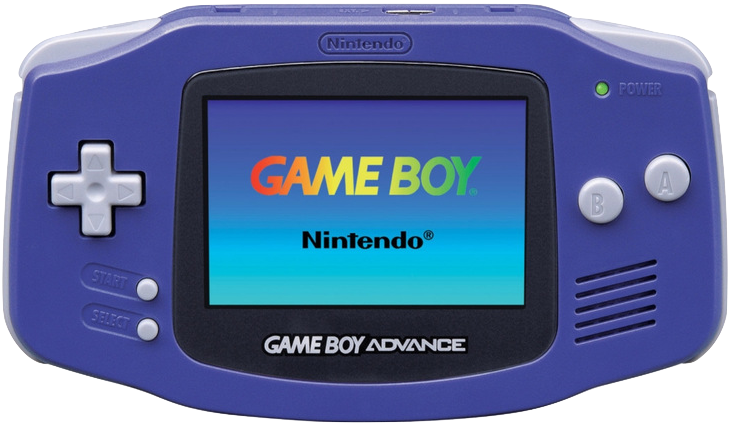
\includegraphics[width=0.5\textwidth]{GameBoyAdvance}
    \caption{Game Boy Advanced - Blue Edition}
    \label{fig:gba}
\end{figure}

Der zentrale Inhalt der Studienarbeit, ist das Reverse Engineering eines solchen Game Boy Advance Emulators. Der genaue Inhalt dieser wird in den n\"achsten Kapiteln zun\"achst eingeschr\"ankt und sp\"ater weiter konkretisiert.

Emulatoren geh\"oren zu einem beliebten Werkzeug der Informatik. Sie bilden ein System oder ein Teilsystem ab. Dabei ist zu beachten, dass diese bekanntes Verhalten nur \enquote{nachahmen}. Genauer ausgef\"uhrt bedeutet dies, dass zum Beispiel bei einem Game Boy Advance Emulator die Software intern anders als auf dem originalen Ger\"at arbeitet. Jedoch kommt es beim Emulieren nicht auf die gleiche Arbeitsweise an, sondern auf das Ergebnis. In diesem konkreten Fall, einen voll funktionsf\"ahigen Nachbau des Game Boys in Software. Mit dem es m\"oglich ist digitalisierte Versionen eines Spieles spielen zu k\"onnen.\newline

\begin{table}[h]
    \centering
    \begin{tabular}{ r | p{10cm} }
        \textbf{CPU} & 16,77 MHz 32 Bit RISC (ARM7TDMI)\newline
              8 Bit CISC CPU (Z80/8080-Derivat) \\
        \hline
        \textbf{Arbeitsspeicher} & 32 KB IRAM (1 cycle/32 bit)\newline
                          + 96 KB VRAM (1-2 cycles)\newline
                          + 256 KB ERAM (6 cycles/32 bit) \\
        \hline
        \textbf{Lautsprecher} & Lautsprecher (Mono), Kopfh\"orer (Stereo) \\
    \end{tabular}
    \caption{Technische Daten des Game Boy Advance \cite{GameBoyTechnischeDaten}}
    \label{table:TechnischeDaten}
\end{table}

\newpage

\subsection{Untersuchungsgegenstand}
\AutorFlorian

In dieser Studienarbeit wird die Fragestellung, wie wird das Soundsystem des Game Boy Advance in einem beliebigen Emulator emuliert, thematisiert. Ein konkreter Emulator wurde nicht vorgegeben. Wir einigten uns demnach auf den Game Boy Advance Emulator \enquote{mGBA}. Dieser stellt im Folgenden unseren zentralen Untersuchungsgegenstand dar.

Die Untersuchung wird in vier Unterthemen gegliedert:

\begin{itemize}
    \item Erstellung eines Beispielprogramms (siehe Abschnitt \ref{Plattformen} und Abschnitt \ref{Softwareentwicklung})
    \item Untersuchung der Fragestellung mit Hilfe eines Beispielprogrammes (siehe Abschnitt \ref{Softwareentwicklung})
    \item Untersuchung der Interaktion des Beispielprogrammes mit dem Emulator (siehe Abschnitt \ref{EmulationGameBoyAdvance})
    \item Untersuchung der Interaktion von Emulator und Betriebssystem (siehe Abschnitt \ref{EmulationSoundsystem})
\end{itemize}

\subsection{Verwendete Software}
\AutorFlorian

\begin{itemize}
    \item \textbf{Betriebssysteme}: Ubuntu 16.0 x64, Windows 10 x64, macOS 10.13.4
    \item \textbf{Disassembler}: IDA Pro
    \item \textbf{Emualtor}: mGBA
    \item \textbf{SDK}: devkitPro
    \item \textbf{IDE's}: Programmer's Notepad, Visual Studio Code, Eclipse, Qt Creator
\end{itemize}

\newpage

% ========== Chapter 2 ==========

\section{Game Boy Advance} \label{GameBoyAdvance}
\AutorFlorianNgoc

\subsection{Hardwareumgebung}
\AutorFlorian

Der Game Boy Advance verf\"ugt \"uber sechs Soundkan\"ale. Vier davon wurden, vor allem aus Gr\"unden der Abw\"artskompatibilit\"at, aus dem Vorg\"anger \enquote{Game Boy Classic} \"ubernommen.

\begin{table}[h]
    \centering
    \begin{tabular}{ r | p{10cm} }
        \textbf{Kanal} & \textbf{Art} \\
        \hline
        1 & Rechteckwellengenerator (square wave generator) \\
        \hline
        2 & Rechteckwellengenerator (square wave generator) \\
        \hline
        3 & Klangerzeuger (Sample-Player) \\
        \hline
        4 & Rauschgenerator (Noise-Generator) \\
        \hline
        A & Direct Sound \\
        \hline
        B & Direct Sound \\
    \end{tabular}
    \caption{\"Ubersicht der Soundkan\"ale des Game Boy Advance}
    \label{table:TechnischeDaten}
\end{table}

% ========== Chapter 2.1.1 ==========

\subsubsection{\"Ubersicht der Audio Register}
\AutorFlorian

Intern besitzt der Game Boy Advance drei Sound-Master-Register. Dort m\"ussen, je nach Einstellungswunsch, ein paar Bits gesetzt werden. Erst dann ist eine Soundwiedergabe oder die generelle Funktionsf\"ahigkeit des Soundsystems m\"oglich. \cite{GameBoySoundsystem}

Der Offset im Folgenden bezieht sich auf die Basisadresse $0x04000000$ und wird in hexadezimaler Schreibweise angegeben. An dieser Stelle muss darauf hingewiesen werden, dass die Bezeichnungen der Register nicht eindeutig sind und sich je nach verwendeter Quelle unterscheiden.

\begin{table}[h]
    \centering
    \begin{tabular}{ c | c | p{10cm} | l }
        \textbf{Offset} & \textbf{Kanal} & \textbf{Funktion} & \textbf{Bezeichnung} \\
        \hline
        $0x060$ & 1 & DMG Sweep control & \verb|SOUND1CNT_L| \\
        \hline
        $0x062$ & 1 & DMG Length, wave and evelope control & \verb|SOUND1CNT_H| \\
        \hline
        $0x064$ & 1 & DMG Frequency, reset and loop control & \verb|SOUND1CNT_X| \\
        \hline
        $0x068$ & 2 & DMG Length, wave and evelope control & \verb|SOUND2CNT_L| \\
        \hline
        $0x06C$ & 2 & DMG Frequency, reset and loop control & \verb|SOUND2CNT_H| \\
    \end{tabular}
    \caption{\"Ubersicht der Sound-Register - Teil 1}
    \label{table:SoundRegister1}
\end{table}

\newpage

\begin{table}[h]
    \centering
    \begin{tabular}{ c | c | p{10cm} | l }    
        \textbf{Offset} & \textbf{Kanal} & \textbf{Funktion} & \textbf{Bezeichnung} \\
        \hline
        $0x070$ & 3 & DMG Enable and wave ram bank control & \verb|SOUND3CNT_L| \\
        \hline
        $0x072$ & 3 & DMG Sound length and output level control & \verb|SOUND3CNT_H| \\
        \hline
        $0x074$ & 4 & DMG Frequency, reset and loop control & \verb|SOUND3CNT_X| \\
        \hline
        $0x078$ & 4 & DMG Length, output level and evelope control & \verb|SOUND4CNT_L| \\
        \hline
        $0x07C$ & 4 & DMG Noise parameters, reset and loop control & \verb|SOUND4CNT_H| \\
        \hline
        $0x080$ & & DMG Master Control & \verb|SOUNDCNT_L| \\
        \hline
        $0x082$ & & Direct Sound Master Control & \verb|SOUNDCNT_H| \\
        \hline
        $0x084$ & & Master Sound Output Control / Status & \verb|SOUNDCNT_X| \\
        \hline
        $0x088$ & & Sound Bias & \verb|SOUNDBIAS| \\
        \hline
        $0x090$ & 3 & DMG Wave RAM Register & \verb|WAVE_RAM0_L| \\
        \hline
        $0x092$ & 3 & DMG Wave RAM Register & \verb|WAVE_RAM0_H| \\
        \hline
        $0x094$ & 3 & DMG Wave RAM Register & \verb|WAVE_RAM1_L| \\
        \hline
        $0x096$ & 3 & DMG Wave RAM Register & \verb|WAVE_RAM1_H| \\
        \hline
        $0x098$ & 3 & DMG Wave RAM Register & \verb|WAVE_RAM2_L| \\
        \hline
        $0x09A$ & 3 & DMG Wave RAM Register & \verb|WAVE_RAM2_H| \\
        \hline
        $0x09C$ & 3 & DMG Wave RAM Register & \verb|WAVE_RAM3_L| \\
        \hline
        $0x09E$ & 3 & DMG Wave RAM Register & \verb|WAVE_RAM3_H| \\
        \hline
        $0x0A0$ & A & Direct Sound FIFO & \verb|FIFO_A_L| \\
        \hline
        $0x0A2$ & A & Direct Sound FIFO & \verb|FIFO_A_H| \\
        \hline
        $0x0A4$ & B & Direct Sound FIFO & \verb|FIFO_B_L| \\
        \hline
        $0x0A6$ & B & Direct Sound FIFO & \verb|FIFO_B_H| \\
    \end{tabular}
    \caption{\"Ubersicht der Sound-Register - Teil 2}
    \label{table:SoundRegister2}
\end{table}

Die in Tabelle \ref{table:SoundRegister1} und in Tabelle \ref{table:SoundRegister2} gelisteten Register sind im mGBA als Felder der Enumeration \textit{GBAIORegisters} (\textit{\$/include/mgba/internal/gba/io.h}) gelistet und entsprechend ihrer Registeradressen belegt. Sie werden unter anderen zur Adressierung des emulierten Speichers verwendet. Als Quelle f\"ur die beiden Tabellen diente neben der \textit{io.h} auch die Webseite \url{http://belogic.com/gba/}, Stand Juni 2018.

\newpage

% ========== Chapter 2.1.2 ==========

\subsubsection{\"Ubersicht der Sound Master Register}
\AutorFlorian

Die Register DMG Master Control, Direct Sound Master Control und Master Sound Output Control / Status bilden die Sound Master Register.

\vspace{5mm}
\large DMG Master Control \label{dmgmastercontrol}
\vspace{2mm}\newline
Hier m\"ussen zun\"achst einige Bits gesetzt werden, bevor eine generelle Verwendung des Soundsystems m\"oglich ist.

\begin{table}[h]
	\centering
    \begin{tabular}{ c | c | p{10cm} | l } 
	    \textbf{Bit} & \textbf{Kanal} & \textbf{Funktion} & \textbf{Bezeichnung} \\
	    \hline
	    0 & 1-4 & Left Volume & \\
	    \hline
	    1 & 1-4 & Left Volume & \\
	    \hline
	    2 & 1-4 & Left Volume & \\
	    \hline
	    3 & & & \\
	    \hline
	    4 & 1-4 & Right Volume & \\
	    \hline
	    5 & 1-4 & Right Volume & \\
	    \hline
	    6 & 1-4 & Right Volume & \\
	    \hline
	    7 & & & \\
	    \hline
	    8 & 1 & Channel 1 Left & \verb|SDMG_LSQR1| \\
	    \hline
	    9 & 2 & Channel 2 Left & \verb|SDMG_LSQR2| \\
	    \hline
	    A & 3 & Channel 3 Left & \verb|SDMG_LWAVE| \\
	    \hline
	    B & 4 & Channel 4 Left & \verb|SDMG_LNOISE| \\
	    \hline
	    C & 1 & Channel 1 Right & \verb|SDMG_RSQR1| \\
	    \hline
	    D & 2 & Channel 2 Right & \verb|SDMG_RSQR2| \\
	    \hline
	    E & 3 & Channel 3 Right & \verb|SDMG_RWAVE| \\
	    \hline
	    F & 4 & Channel 4 Right & \verb|SDMG_RNOISE| \\
	\end{tabular}
	\caption{DMG Master Control Register}
	\label{table:DmgMasterControlRegister}
\end{table}

\newpage

\vspace{5mm}
\large Direct Sound Master Control \label{directsoundmastercontrol}
\vspace{2mm}\newline
Dieses Register kontrolliert die Lautst\"arke der DMG Kan\"ale und aktiviert diese. Die Einstellungen k\"onnen separiert voneinander f\"ur den linken und rechten Lautsprecher vorgenommen werden.

\begin{table}[h]
	\centering
    \begin{tabular}{ c | c | p{10cm} | l } 
	    \textbf{Bits} & \textbf{Name} & \textbf{Funktion} & \textbf{Bezeichnung} \\
	    \hline
	    0-1 & DMGV & DMG Volume Ratio & \\
	        &      & 00: 25\% & \verb|SDS_DMG25| \\
	        &      & 01: 50\% & \verb|SDS_DMG50| \\
	        &      & 10: 100\% & \verb|SDS_DMG100| \\
	        &      & 11: forbidden \\
	    \hline
	    2 & AV & Direct Sound A Volume Ratio & \\
	      &    & 50\% if clear & \verb|SDSA50| \\
	      &    & 100\% if set  & \verb|SDSA100| \\
        \hline
	    3 & BV & Direct Sound B Volume Ratio & \\
	      &    & 50\% if clear & \verb|SDSB50| \\
	      &    & 100\% if set  & \verb|SDSB100| \\
	    \hline
	    4-7 & & & \\
	    \hline
	    8 & AR & Direct Sound A enable Direct Sound on Right speaker & \verb|SDS_AR| \\
	    \hline
	    9 & AL & Direct Sound A enable Direct Sound on Left speaker & \verb|SDS_AL| \\
	    \hline
	    A & AT & Direct Sound A Timer. & \\
	       &   & Use timer 0 (if clear) for Direct Sound A & \verb|SDS_ATMR0| \\
	       &   & Use timer 1 (if set) for Direct Sound A & \verb|SDS_ATMR1| \\
	    \hline
	    B & AF & FIFO reset for Direct Sound A & \verb|SDS_ARESET| \\
	    \hline
	    C & BR & Direct Sound B enable Direct Sound on Right speaker & \verb|SDS_BR| \\
	    \hline
	    D & BL & Direct Sound B enable Direct Sound on Left speaker & \verb|SDS_BL| \\
	    \hline
	    E & BT & Direct Sound B Timer. & \\
	       &   & Use timer 0 (if clear) for Direct Sound B & \verb|SDS_BTMR0| \\
	       &   & Use timer 1 (if set) for Direct Sound B & \verb|SDS_BTMR1| \\
	    \hline
	    F & BF & FIFO reset for Direct Sound B & \verb|SDS_BRESET| \\
	\end{tabular}
	\caption{Direct Sound Master Control Register}
	\label{table:DirectSoundMasterControlRegister}
\end{table}

Wenn DMA f\"ur Direct Sound verwendet wird, dann wird DMA den FIFO-Puffer zur\"ucksetzen, nachdem er verwendet wurde.






	
\newpage
	
\vspace{5mm}
\large Master Sound Output Control / Status \label{mastersoundoutputcontrol}
\vspace{2mm}\newline
Aus diesem Register kann zu einem der Status der einzelnen DMG Kan\"ale ausgelesen werden und zum Anderen die generelle Soundausgabe aktiviert werden. Dazu muss das Bit 7 gesetzt werden.

\begin{table}[h]
	\centering
    \begin{tabular}{ c | c | p{10cm} | l } 
	    \textbf{Bits} & \textbf{Name} & \textbf{Funktion} & \textbf{Bezeichnung} \\
	    \hline
	    0 & 1A & Channel 1 is active and currently playing. & \verb|SSTAT_SQR1| \\
	    \hline
	    1 & 2A & Channel 2 is active and currently playing. & \verb|SSTAT_SQR2| \\
	    \hline
	    2 & 3A & Channel 3 is active and currently playing. & \verb|SSTAT_WAVE| \\
	    \hline
	    3 & 4A & Channel 4 is active and currently playing. & \verb|SSTAT_NOISE| \\
	    \hline
	    4-6 & & & \\
	    \hline
	    7 & MSE & Master Sound Enable & \verb|SSTAT_DISABLE| \\
	      &     & Must be set if any sound is to be heard at all. Set this before you do anything; otherwise other sound registers can't be accessed (see GBATek for more details). & \verb|SSTAT_ENABLE| \\
	    \hline
	    8-F & & & \\
	\end{tabular}
	\caption{Master Sound Output / Status Register}
	\label{table:MasterSoundOutputControlStatusRegister}
\end{table}

Die Bits 0-3 geben ausschlie{\ss}lich dar\"uber Auskunft, welcher Kanal aktuelle bespielt wird und nicht ob dieser eingeschaltet ist. Zum Ein- und Ausschalten eines Kanals dient das DMG Master Control Register (siehe Abschnitt \ref{dmgmastercontrol}).




\newpage

% ========== Chapter 2.2 ==========

\subsection{Plattformen} \label{Plattformen}
\AutorNgoc

% ========== Chapter 2.2.1 ==========

\subsubsection{DevkitPro}
\AutorNgoc

% ========== Chapter 2.2.2 ==========

\subsubsection{BeLogic}
\AutorNgoc

% ========== Chapter 2.2.3 ==========

\subsubsection{MaxMod}
\AutorNgoc

% ========== Chapter 2.2.4 ==========

\subsubsection{Snappy}
\AutorNgoc

% ========== Chapter 2.3 ==========

\subsection{Softwareentwicklung} \label{Softwareentwicklung}
\AutorNgoc

% ========== Chapter 2.3.1 ==========

\subsubsection{API zur Audioverarbeitung}
\AutorNgoc

% ========== Chapter 2.3.2 ==========

\subsubsection{Audiodaten im Speicher}
\AutorNgoc

% ========== Chapter 2.3.3 ==========

\subsubsection{Snappy - \enquote{Audio-Reflektor}}
\AutorNgoc

% ========== Chapter 2.3.4 ==========

\subsubsection{Untersuchung des Assemblers}
\AutorNgoc


\newpage

% ========== Chapter 3 ==========

\section{Emulation mittels mGBA} \label{EmulationMittelsMGBA}
\AutorDominikFlorian

% ========== Chapter 3.1 ==========

\subsection{Was ist der mGBA?}
\AutorDominik

% ========== Chapter 3.2 ==========

\subsection{Emulation des Game Boy Advance} \label{EmulationGameBoyAdvance}
\AutorDominikFlorian

Die Anwendung \enquote{mGBA} wurde von den Entwicklern mit dem GUI-Toolkit Qt realisiert. Qt erm\"oglicht die plattformunabh\"angige Entwicklung von Anwendungen mit grafischer Benutzeroberfl\"ache und basiert auf der Sprache C++. Damit ist es Entwicklern auch m\"oglich, bereits realisierte Basis-Software problemlos zu integrieren.

% ========== Chapter 3.2.1 ==========

\subsubsection{Abgrenzung der Untersuchung}
\AutorFlorian

F\"ur die Untersuchung, wie der Emulator mit dem Betriebssystem interagiert, wird im Folgenden nur auf die daf\"ur ben\"otigten Klassen, Methoden und Konzepte eingegangen. Dabei liegt der Fokus ausschlie{\ss}lich auf Abl\"aufe die zur Emulation des Soundsystems notwendig sind.

\subsubsection{Start des Emulators}
\AutorDominik

\subsubsection{Initialisierung des \enquote{mCore}}
\AutorDominik

\subsubsection{Laden des ROM}
\AutorDominik

\subsubsection{Starten des ROM}
\AutorDominik

\subsubsection{Ausf\"uhrung des ROM}
\AutorDominik










%\subsubitem{Start der Anwendung}
%\AutorDominik

Wie \"ublich beginnt auch beim mGBA die Anwendung in der globalen \verb|main|-Methode (\textit{\$/src/platform/qt/main.cpp}). Diese initialisiert den \textbf{ConfigController} mittels \verb|argc| und \verb|argv|. Anschlie{\ss}end wird eine neue Instanz der Klasse \textbf{GBAApp} ebenfalls mit \verb|argc| und \verb|argv|, sowie dem vorinitialisierten \verb|configController| initialisiert. Die weitere Logik der \verb|main|-Methode dient der Initialisierung und Lokalisierung einer \textbf{Window}-Instanz zur Anzeige der mGBA GUI. Die dabei erzeugte \textbf{Window}-Instanz wird w\"ahrenddessen dazu aufgefordert die Einstellungen aus dem bereits initialisierten \verb|configController| zu laden. Hierzu wird die Methode \verb|loadConfig()| der \textbf{Window}-Klasse verwendet.

\vspace{5mm}
\large ConfigController \normalsize(\textit{\$/src/platform/qt/ConfigController.h \& .cpp})
\vspace{2mm}\newline
Im Konstruktor der \textbf{ConfigController}-Klasse werden eventuell vorhandene Einstellungen aus einer \enquote{qt.ini} oder \enquote{config.ini} geladen und Standard-Werte der Membervariable \verb|m_opts| vom Typen der \textbf{mCoreOptions}-Struktur (\textit{\$/include/mgba/core/config.h}) festgelegt, siehe Snippet \ref{list:ConfigController_ctor}.

\vspace{5mm}
\begin{lstlisting}[language=C++, caption={Ausschnitt aus dem Konstruktor der ConfigController-Klasse}, label={list:ConfigController_ctor}]
    ...
	m_opts.audioSync = GameController::AUDIO_SYNC;
	m_opts.audioBuffers = 1536;
	m_opts.sampleRate = 44100;
	m_opts.volume = 0x100;
	...
\end{lstlisting}

Alle im \textbf{ConfigController} enthaltenen Einstellungen werden im Laufe der Anwendung je nach Bedarf entweder \"uber die \verb|options()|-Methode oder \"uber die \verb|config()|-Methode abgerufen. Dabei wird bei der ersten Methode eine \textbf{mCoreOptions}-Struktur (\textit{\$/include/mgba/core/config.h}) und bei der zweiten Methode eine \textbf{mCoreConfig}-Struktur (\textit{\$/include/mgba/core/config.h}) bereitgestellt. W\"ahrend die \textbf{mCoreConfig}-Struktur auschlie{\ss}lich eine Abstraktion der konfigurierten Werte, der Standardwerte und der \"uberschriebenen Werte bietet, stellt die \textbf{mCoreOptions}-Struktur alle verf\"ugbaren Einstellungen direkt als typisierte Felder bereit.

\vspace{5mm}
\large GBAApp \normalsize(\textit{\$/src/platform/qt/GBAApp.h \& .cpp})
\vspace{2mm}\newline
Im Konstruktor der \textbf{GBAApp}-Klasse wird der lokale \verb|m_configController| mit dem \"ubergebenen initialisiert und der Treiber der \textbf{AudioProcessor}-Klasse mittels \verb|AudioProcessor.setDriver(...)| festgelegt. Der \textbf{AudioProcessor.Driver} (eine Enumeration) legt dabei fest, ob entweder die \textbf{AudioProcessor}-Spezialisierung \textbf{AudioProcessorQt} oder \textbf{AudioProcessorSDL} mittels \verb|AudioProcessor.create()|-Aufruf erstellt wird. Der zu verwendende \textbf{AudioProcessor.Driver} wird dabei durch den \textbf{ConfigController} \"uber die Option \enquote{audioDriver} bereitgestellt.

\vspace{5mm}
\large Window \normalsize(\textit{\$/src/platform/qt/Window.h \& .cpp})
\vspace{2mm}\newline
Im Konstruktor der \textbf{Window}-Klasse wird die lokale \verb|m_config| mit dem \"ubergebenen \textbf{ConfigController} (\verb|config|-Parameter) und der lokale \verb|m_inputController| initialisiert. Daraufhin wird eine neue Instanz der \textbf{GameController}-Klasse erzeugt, in der Membervariablen \verb|m_controller| gespeichert und der \verb|m_inputController| an die \textbf{GameController}-Instanz mittels \verb|m_controller.setInputController(...)| \"ubergeben. Weiter stellt der Konstruktor der \textbf{Window}-Klasse Verbindungen mittels Qt Signals \& Slots zwischen den folgenden Methoden her:

\begin{itemize}
    \item \verb|Window.audioBufferSamplesChanged| $\rightarrow$ \verb|m_controller::setAudioBufferSamples|
    \item \verb|Window.sampleRateChanged| $\rightarrow$ \verb|m_controller.setAudioSampleRate|
\end{itemize}

Als letzte Anweisung des Konstruktors wird die lokale \verb|setupMenu()|-Methode der \textbf{Window}-Klasse aufgerufen. Neben diversen Men\"ueintr\"agen erzeugt diese Methode auch Men\"upunkte zur Interaktion mit dem emulierten Soundsystem. Besonders interessant ist dabei auch der Men\"upunkt \enquote{Record output...}, welcher mittels Qt Signals \& Slots mit der Methode \verb|openVideoWindow()| der \textbf{Window}-Klasse verbunden wird. Bei Ausf\"uhrung der \verb|openVideoWindow()|-Methode wird eine neue Instanz der \textbf{VideoView}-Klasse erzeugt (falls nicht bereits geschehen) und die folgenden Methoden mittels Qt Signals \& Slots mit Methoden der \textbf{GameController}-Klasse verbunden. Zum Ende der Methode wird das \textit{QWidget} \textbf{VideoView} noch zur Anzeige gebracht.

\begin{itemize}
    \item \verb|VideoView.recordingStarted| $\rightarrow$ \verb|m_controller.setAVStream|
    \item \verb|VideoView.recordingStopped| $\rightarrow$ \verb|m_controller.clearAVStream|
\end{itemize}


Durch den Aufruf der \verb|loadConfig()|-Methode wird wiederum die Methode \verb|reloadConfig()| der \textbf{Window}-Klasse aufgerufen. Diese vermittelt unter anderen die aktuelle \textbf{mCoreConfig}-Struktur der \verb|m_config| (vom Typen \textbf{ConfigController}) an den \verb|m_controller| (vom Typen \textbf{GameController}) mittels \verb|setConfig()|-Methode der \textbf{GameController}-Klasse.

\vspace{5mm}
\large VideoView \normalsize(\textit{\$/src/platform/qt/VideoView.h \& .cpp})
\vspace{2mm}\newline
Bei der Instanziierung der \textbf{VideoView}-Klasse verwendet der Konstruktor die globale Methode \textbf{FFmpegEncoderInit} (\$/src/feature/ffmpeg/ffmpeg-encoder.c) zur Initialisierung der Membervariablen \verb|m_encoder|. Die f\"ur die Audio-/Videoausgabe verwendete Struktur vom Typen \textbf{FFmpegEncoder} (\$/src/feature/ffmpeg/ffmpeg-encoder.c) wird beim Aufruf der Instanzmethode \verb|startRecording()| der \textbf{VideoView}-Klasse mttels globaler \textbf{FFmpegEncoderOpen} Methode so final konfiguriert, dass der Encoder die bei der Emulation anfallenden Audio-/Videodaten aufzeichnet. Zum Abschluss der \textbf{startRecording()}-Methode wird das Qt Signal \verb|recordingStarted| mit dem Feld \verb|d| vom Typen der Struktur \textbf{mAVStream} der \verb|m_encoder| Membervariablen als Parameter gesendet. Dieses Signal endet schlie{\ss}lich in einen Aufruf der \verb|setAVStream|-Methode der \textbf{GameController}-Instanz \verb|m_controller| der \textbf{Window}-Klasse.

\vspace{5mm}
\large GameController \normalsize(\textit{\$/src/platform/qt/GameController.h \& .cpp})
\vspace{2mm}\newline
Im Konstruktor der \textbf{GameController}-Klasse wird die lokale \verb|m_audioProcessor| Membervariable mit dem Ergebnis des \verb|AudioProcessor.create()|-Aufrufs initialisiert. Daraufhin erfolgt das Setup der Membervariable \verb|m_threadContext| vom Typen der \textbf{mCoreThread}-Struktur. Hierbei wird unter anderen das \verb|startCallback|, \verb|cleanCallback| und das \verb|userData| Feld der Kontextvariablen entsprechend belegt. Abschlie{\ss}end werden die folgenden Methoden mittels Qt Signals \& Slots miteinander verbunden:

\begin{itemize}
    \item \verb|GameController.gamePaused| $\rightarrow$ \verb|m_audioProcessor.pause|
    \item \verb|GameController.gameStarted| $\rightarrow$ \verb|m_audioProcessor.setInput|
\end{itemize}


%\subsubsection{Laden und Starten eines ROM}
%\AutorDominik

W\"ahlt der mGBA-Anwender im Men\"u den Punkt \enquote{Load ROM...}, wird hierf\"ur die Methode \verb|selectROM()| der \textbf{Window}-Klasse ausgef\"uhrt. Nach erfolgter Auswahl einer entsprechend unterst\"utzten Datei, wird die Methode \verb|loadGame(path)|  der lokalen \textbf{GameController}-Instanz (\verb|m_controller|) mit dem Pfad zur ausgew\"ahlten ROM-Datei aufgerufen. Diese f\"uhrt nach einigen Vorabaktionen die Methode \verb|openGame()| der \textbf{GameController}-Instanz aus. Mittels globaler \textbf{mCoreFind}-Methode (\textit{\$/src/core/core.c}) wird der vom Format der ROM-Datei abh\"angige \enquote{Core} ermittelt und erstellt. Handelt es sich bei der ROM-Datei um ein Game Boy Advance (kurz \enquote{GBA}) Speicherabbild, wird die globale \textbf{GBACoreCreate}-Methode (\textit{\$/src/gba/core.c}) dazu verwendet den Speicher f\"ur die Struktur \textbf{GBACore} (\textit{\$/src/gba/core.c}) zu allokieren. Das dabei implizit allokierte \textbf{mCore}-Feld \verb|d| wird daraufhin mit diversen Funktionszeigern zu globalen Methoden mit dem Prefix \textbf{{\_}GBA} beziehungsweise \textbf{{\_}GBACore} initialisiert. Das auf diese Weise konfigurierte \verb|d|-Feld wird dann von der globalen \textbf{GBACoreCreate}-Methode zur\"uckgeliefert und im Feld \verb|mCoreThread.core| der lokalen Membervariable \verb|m_threadContext| der \textbf{GameController}-Instanz gespeichert.

\vspace{5mm}
\large {\_}GBACoreInit \normalsize(\textit{\$/src/gba/core.c})
\vspace{2mm}\newline
Der erste der zuvor festgelegten Funktionszeiger der daraufhin verwendet wird ist der der Funktion auf die im Feld \verb|init| verwiesen wird. Nach Durchlaufen der globalen \textbf{GBACoreCreate}-Methode ist das die globale Methode \textbf{{\_}GBACoreInit}. Die globale Methode initialisiert die Felder \verb|cpu| und \verb|board| des \textbf{mCore}. Hierzu wird f\"ur das Feld \verb|cpu| die Struktur \textbf{ARMCore} (\textit{\$/include/mgba/internal/arm/arm.h}) und f\"ur das Feld \verb|board| die Struktur \textbf{GBA} (\textit{\$/include/mgba/internal/gba/gba.h}) verwendet. Nach der Initialisierung einzelner weiterer Felder wird dann die globale Methode \textbf{GBACreate} (\textit{\$/src/gba/gba.c}) mit den Verweis auf die zuvor initialisierte \verb|board|-Variable vom Typen der \textbf{GBA}-Struktur aufgerufen. Diese legt unter anderen als Wert f\"ur das \verb|init|-Feld des \verb|d|-Feldes vom Typen der \textbf{mCPUComponent}-Struktur der \verb|board|-Variablen die globale Methode \textbf{GBAInit} (\textit{\$/src/gba/gba.c}) fest. \sout{Im weiteren Verlauf der \textbf{{\_}GBACoreInit}-Methode wird schlie{\ss}lich noch die globale Methode \textbf{ARMInit} aufgerufen und ihr dabei die zuvor initialisierte cpu-Variable vom Typen der \textbf{ARMCore}-Struktur \"ubergeben.} Anschlie{\ss}end wird in Folge der Aufrufe der globalen Methoden \textbf{ARMSetComponents} (\textit{\$/src/arm/arm.c}) und \textbf{ARMInit} (\textit{\$/src/arm/arm.c}) die zuvor auf dem \verb|init|-Feld des \verb|d|-Feldes der \verb|board|-Variablen die globale Methode \textbf{GBAInit} aufgerufen.

\vspace{5mm}
\large GBAInit \normalsize(\textit{\$/src/gba/gba.c})
\vspace{2mm}\newline
In dieser Low-Level Init-Routine werden alle virtuellen Hardwarekomponenten des \textbf{mCore} initialisiert und mit weiteren globalen Methoden verlinkt. Dazu geh\"ohrt unter anderen das Setup des Interrupt-Handlers, welcher \"uber das Feld \verb|irqh| des \verb|cpu|-Feldes der \textbf{GBA}-Instanz an die globale Methode \textbf{GBAInterruptHandlerInit} \"ubergeben wird. Nach der Initialisierung des Interrupt-Handlers folgt die Initialisierung des Speichers des \textbf{GBA} mittels globaler \textbf{GBAMemoryInit}-Methode. Darauf folgt das Setup der \enquote{Audio}-Peripherie des \textbf{GBA} mit Hilfe der globalen Methode \textbf{GBAAudioInit}.

\vspace{5mm}
\large GBAInterruptHandlerInit \normalsize(\textit{\$/src/gba/gba.c})
\vspace{2mm}\newline
Die einzige Aufgabe dieser Methode ist es die \textbf{ARMInterruptHandler}-Struktur (\textit{\$/include/mgba/internal/arm/arm.h}) des \textbf{GBA} zu initialisieren. Hierzu legt die Methode entsprechende Funktionszeiger f\"ur die einzelnen Service-Routinen der Interrupt-Handler-Struktur fest.

\vspace{5mm}
\begin{lstlisting}[language=C++, caption={Ausschnitt aus der \textbf{GBAInterruptHandlerInit}-Methode}, label={list:GBAInterruptHandlerInit}]
    irqh->reset = GBAReset;
    irqh->processEvents = GBAProcessEvents;
    irqh->swi16 = GBASwi16;
    irqh->swi32 = GBASwi32;
    ...
\end{lstlisting}

\vspace{5mm}
\large GBAMemoryInit \normalsize(\textit{\$/src/gba/memory.c})
\vspace{2mm}\newline
Neben den diversen Initialisierungsoperationen und Aufrufen weiterer Subroutinen zur Initialisierung des \verb|memory|-Feldes der \enquote{CPU} \"uber das \verb|cpu|-Feld des \textbf{GBA} legt auch diese Methode entsprechende Funktionszeiger f\"ur die einzelnen Speicherzugriffe auf der \textbf{ARMMemory}-Struktur (\textit{\$/include/mgba/internal/arm/arm.h}) fest. Die im folgenden Snippet gezeigten Zeilen sind f\"ur die Untersuchtung der Emulation des Soundsystems relevant.

\vspace{5mm}
\begin{lstlisting}[language=C++, caption={Ausschnitt aus der \textbf{GBAMemoryInit}-Methode}, label={list:GBAMemoryInit}]
    ...
    cpu->memory.load32 = GBALoad32;
    cpu->memory.load16 = GBALoad16;
    cpu->memory.load8 = GBALoad8;
    cpu->memory.loadMultiple = GBALoadMultiple;
    cpu->memory.store32 = GBAStore32;
    cpu->memory.store16 = GBAStore16;
    cpu->memory.store8 = GBAStore8;
    cpu->memory.storeMultiple = GBAStoreMultiple;
    cpu->memory.stall = GBAMemoryStall;
    ...
\end{lstlisting}

\vspace{5mm}
\large GBAAudioInit \normalsize(\textit{\$/src/gba/audio.c})
\vspace{2mm}\newline
Die globale \textbf{GBAAudioInit}-Methode ist f\"ur den vollen Setup der \textbf{GBAAudio}-Struktur (\textit{\$/include/mgba/internal/gba/audio.h}) der \textbf{GBA}-Instanz verantwortlich. Neben diversen Audio-Parametern werden auch ben\"otigte \textbf{mTimingEvent}-Strukturen initialisiert. Diese Event-Strukturen dienen dem Scheduler sp\"ater bei der quasi-parallelen Verarbeitung der Audiodaten. Die daf\"ur eigens definierten Events werden mit entsprechenden Callback-Routinen verlinkt, welche die verz\"ogerte / parallele Verarbeitung der Audiodaten durchf\"uhren. Zusammen mit der ebenfalls globalen Methode \textbf{GBAudioInit} werden w\"ahrend der Ausf\"uhrung der Methode die folgenden Events konfiguriert.

\begin{table}[h]
    \centering
    \begin{tabular}{ r | p{3cm} | c | p{7cm} }
        \textbf{Event} & \textbf{Priorit\"at} & \textbf{Kanal} & \textbf{Callback} \\
        \hline
        GB(A) Audio Sample & $0x18$ & & \verb|_sample| \\
        \hline
        GB  Audio Frame Sequencer & $0x10$ & & \verb|_updateFrame| \\
        \hline
        GB Audio Channel 1 & $0x11 \rightarrow 0x18$ & 1 & \verb|_updateChannel1|  \\
        \hline
        GB Audio Channel 2 & $0x12$ & 2 & \verb|_updateChannel2| \\
        \hline
        GB Audio Channel 3 & $0x13$ & 3 & \verb|_updateChannel3| \\
        \hline
        GB Audio Channel 3 Memory & $0x14$ & 3 & \verb|_fadeChannel3| \\
        \hline
        GB Audio Channel 4 & $0x15$ & 4 & \verb|_updateChannel4| \\
    \end{tabular}
    \caption{\"Ubersicht der Events der Soundkan\"ale des Game Boy Advance}
    \label{table:SoundEvents}
\end{table}


\vspace{5mm}
\large {\_}GBACoreSetAudioBufferSize \normalsize(\textit{\$/src/gba/core.c})
\vspace{2mm}\newline
Anschlie{\ss}end wird mit Hilfe der globalen Methode \textbf{mCoreLoadForeignConfig} (\textit{\$/src/core/core.c}) die Konfiguration der \textbf{ConfigController}-Instanz, die durch die \textbf{Window}-Klasse an den \textbf{GameController} \"ubertragen wurde, auf den \textbf{mCore} des \verb|core|-Feldes der Membervariablen \verb|m_threadContext| angewendet. Hierbei wird unter anderen die Funktion auf die im Feld \verb|setAudioBufferSize| verwiesen wird aufgerufen. Nach Durchlaufen der globalen \textbf{GBACoreCreate}-Methode ist das die globale Methode \textbf{{\_}GBACoreSetAudioBufferSize}. Sie leitet den Aufruf direkt weiter an die globale Methode \textbf{GBAAudioResizeBuffer} unter Verwendung des \verb|audio|-Feldes der \textbf{GBAAudio}-Struktur des \verb|board|-Felds der \textbf{mCore}-Struktur.

\vspace{5mm}
\large {\_}GBACoreLoadConfig \normalsize(\textit{\$/src/gba/core.c})
\vspace{2mm}\newline
Nachdem die Funktion auf die im Feld \verb|setAudioBufferSize| verwiesen wird aufgerufen wurde, wird von der globalen Methode \textbf{mCoreLoadForeignConfig} die allgemeine Funktion auf die im Feld \verb|loadConfig| verwiesen wird aufgerufen. Nach Durchlaufen der globalen \textbf{GBACoreCreate}-Methode ist das die globale Methode \textbf{{\_}GBACoreLoadConfig}. Sie \"ubernimmt im Wesentlichen die Konfiguration f\"ur das Mastervolume des \verb|audio|-Feldes der \textbf{GBAAudio}-Struktur des \verb|board|-Felds der \textbf{mCore}-Struktur.

\vspace{5mm}
\large {\_}GBACoreLoadROM \normalsize(\textit{\$/src/gba/core.c})
\vspace{2mm}\newline
Auf die vorangegangene Konfiguration des \textbf{mCore} wird schlie{\ss}lich der ROM in den \enquote{Core} geladen. Hierzu verwendet die \textbf{GameController}-Instanz die Funktion auf die im Feld \verb|loadROM| verwiesen wird. Nach Durchlaufen der globalen \textbf{GBACoreCreate}-Methode ist das die globale Methode \textbf{{\_}GBACoreLoadROM}. Sie dient dem finalen Setup der virtuellen Hardwarekonfiguration des \textbf{mCore} sowie der Initialisierung des virtuellen Prozessspeichers im \verb|memory|-Feld des \verb|board|-Feldes der \textbf{mCore}-Instanz.

\vspace{5mm}
\large {\_}GBACoreSetAVStream \normalsize(\textit{\$/src/gba/core.c})
\vspace{2mm}\newline
Bevor mit der eigentlichen Emulation begonnen wird, wird nun noch der Audio-/Videostream in Form der \textbf{mAVStream}-Struktur als \verb|m_stream|-Membervariable der \textbf{GameController}-Instanz an den \textbf{mCore} \"ubergeben. Diese geschieht durch Aufruf der Funktion auf die im Feld \verb|setAVStream| verwiesen wird. Nach Durchlaufen der globalen \textbf{GBACoreCreate}-Methode ist das die globale Methode \textbf{{\_}GBACoreSetAVStream}. Diese Methode geht hierbei lediglich dazu \"uber den \textbf{mAVStream}-Verweis im \verb|stream|-Feld des \verb|board|-Feldes der \textbf{mCore}-Instanz zu speichern.

\vspace{5mm}
\large {\_}GBACoreEnableAudioChannel \normalsize(\textit{\$/src/gba/core.c})
\vspace{2mm}\newline
Aufgabe dieser globalen Methode ist es dem \verb|board|-Feld des \textbf{mCore} mittels gegebener Parameter zu konfigurieren. Das hierbei vorgenommene Setup bezieht sich auschlie{\ss}lich auf das \verb|audio|-Feld des \verb|board|-Felds vom Typen der \textbf{GBA}-Struktur. Die dabei vorgenommenen \"Anderungen beziehen sich somit nur auf Felder der \textbf{GBAAudio}-Struktur.

\vspace{5mm}
\large mCoreThreadStart \normalsize(\textit{\$/src/core/thread.c})
\vspace{2mm}\newline
Nach Abschluss des vollst\"andigen Setups des \textbf{mCore} wird die im \verb|m_threadContext.core| gespeicherte Instanz samt \verb|m_threadContext| an die globale Methode \textbf{mCoreThreadStart} \"ubergeben. Bevor aber die Methode den eigentlichen Thread erzeugt initialisiert sie diverse Mutex- sowie Condition-Instanzen zur Synchronisation der Thread-\"ubergreifenden Operationen. Von besonderer Bedeutung sind hierbei der Mutex \verb|audioBufferMutex| und die Condition \verb|audioRequiredCond|. Beide Felder sind Teil der \textbf{mCoreSync}-Struktur des \verb|theadContext|-Parameters vom Typen \textbf{mCoreThread}.

Sind alle Bedingungen f\"ur das Multithreading erf\"ullt, legt die Methode mittels globaler \textbf{ThreadCreate}-Methode (\textit{\$/include/mgba-util/platform/\{os\}/threading.h}) den Emulations-Thread an. Als \textbf{ThreadEntry} wird dabei die globale Methode \textbf{{\_}mCoreThreadRun} und als \verb|context|-Parameter ein Verweis auf den \textbf{mCoreThread} alias \verb|threadContext| verwendet. Der Verweis auf den so erzeugten Thread wird schlie{\ss}lich noch im \verb|thread|-Feld des \verb|threadContext|-Parameters gespeichert.

\newpage

\vspace{5mm}
\large {\_}mCoreThreadRun \normalsize(\textit{\$/src/core/thread.c})
\vspace{2mm}\newline
Bevor nun mit der eigentlichen Ausf\"uhrung des Prozesses begonnen wird, nimmt die globale \textbf{{\_}mCoreThreadRun} noch ein paar Vorkehrungen f\"ur die Threadinteraktion mittels Callback-Routinen vor. Darauf folgt der Aufruf der im Feld \verb|startCallback| des \verb|threadContext|-Parameters hinterlegten Methode. Dabei wird die durch die \textbf{GameContoller}-Klasse definierte anonyme Methode mit \verb|threadContext|-Parameter aufgerufen. W\"ahrend der Ausf\"uhrung des Start-Callbacks stellt der \textbf{GameController} sicher, dass im \textbf{mCore} (im \verb|core|-Feld des \verb|threadContext|-Parameters) die korrekten Audio-Kan\"ale ein- beziehungsweise ausgeschaltet sind. Hierzu verwendet der \textbf{GameController} die Funktion auf die im Feld \verb|enableAudioChannel| verwiesen wird. Nach Durchlaufen der globalen \textbf{GBACoreCreate}-Methode ist das die globale Methode \textbf{{\_}GBACoreEnableAudioChannel}.

Abgeschlossen wird der Code der Callback-Routine mit dem dynamischen Ausl\"osen der Signale \textbf{gameStarted} und \textbf{startAudio} der \textbf{GameController}-Instanz die f\"ur den \"ubergebenen \verb|threadContext| zust\"andig ist. W\"ahrend \textbf{gameStarted} auf die \verb|setInput()|-Methode der \verb|m_audioProcessor|-Instanz im \textbf{GameController} weiterleitet, um den aktuellen \textbf{mCoreThread} der \textbf{AudioProcessor}-Instanz mitzuteilen, f\"uhrt der Aufruf des \textbf{startAudio}-Signals zum Aufruf der \verb|start()|-Methode der \verb|m_audioProcessor|-Instanz im \textbf{GameController}.

Wurde auch alle weiteren Callback-Routinen durchlaufen, beginnt die Ausf\"uhrung des Prozesses durch stetigen Aufruf der Funktion auf die im Feld \verb|runLoop| verwiesen wird. Nach Durchlaufen der globalen \textbf{GBACoreCreate}-Methode ist das die globale Methode \textbf{{\_}GBACoreRunLoop}. Dies geschieht solange, wie sich der Thread im Zustand kleiner/gleich \verb|THREAD_MAX_RUNNING| befindet.


%\subsubsection{Ausf\"uhrung eines ROM}
%\AutorDominik

Nach Durchlaufen der Setup-Phase bestehend aus dem Einrichten der notwendigen Strukturen und dem Laden des Prozessspeichers, kann der Inhalt des ROMs gem\"a{\ss} dem bekannten Instruction-Set eines ARM-Prozessors abgerarbeitet werden. Hierbei wird jede Anweisung im ROM sequentiell eine nach der anderen ausgewertet und ausgef\"uhrt. Die dabei im ROM beschriebenen Assembler Befehle f\"ur die ARM-Architektur, werden durch entsprechende Methoden abgearbeitet, welche das Verhalten der Plattform so emulieren, als ob der Prozess auf einem physikalichen ARM ausgef\"uhrt werden w\"urde.

\vspace{5mm}
\large {\_}GBACoreRunLoop \normalsize(\textit{\$/src/gba/core.c})
\vspace{2mm}\newline
Die bereits im vorangegangenen Abschnitt erw\"ahnte globale Methode ist f\"ur die Ausf\"uhrung der einzelnen Assembler Anweisungen im geladenen ROM zust\"andig. Hierzu bedient sie sich der ebenfalls globalen Methode \textbf{ARMRunLoop} und \"ubergibt dieser dabei die Kontrolle \"uber die \enquote{CPU}.

\vspace{5mm}
\large ARMRunLoop \normalsize(\textit{\$/src/arm/arm.c})
\vspace{2mm}\newline
Mit Hilfe der \"ubergebenen \enquote{CPU} in Form der \textbf{ARMCore}-Struktur f\"uhrt die Methode die Assembler-Anweisungen Schritt f\"ur Schritt aus. Dabei ber\"ucksichtigt sie die Anzahl der auszuf\"uhrenden Anweisungen in Abh\"angigkeit zur Ausf\"uhrung des n\"achsten Events. Bis es zur einer Abarbeitung von Events kommt wird je Zyklus die globale Methode \textbf{ARMStep} ausgef\"uhrt. Entspricht die Anzahl der vollzogenen Zyklen dem Zyklus eines anstehenden Events, wird die weitere Verarbeitung unterbrochen und dem Interrupt-Service-Routinen-Handler Zeit gegeben die anstehenden Events abzuarbeiten.

\vspace{5mm}
\large ARMStep \normalsize(\textit{\$/src/arm/arm.c})
\vspace{2mm}\newline
Entsprechend der Natur von Software welche auf Hardware-Level in Form von Assembler-Befehlen ausgef\"uhrt wird, holt auch diese Methode stets den \textbf{OpCode} des als n\"achstes auszuf\"uhrenden Befehls aus dem Prefech-Speicher der \textbf{MMU}. Basierend auf den Wert des \textbf{OpCodes} wird aus einem global definierten und mittels Makros gef\"ulltem Array der Zeiger zur Funktion ermittelt, welche f\"ur die Emulation des Assembler-Befehls verantwortlich ist.

Die zur Ausf\"uhrung per Makro definierten Routinen vollziehen dabei nicht auschlie{\ss}lich einfache Delegationsarbeit zu global definierten Methoden deren Funktionszeiger in diversen Feldern des \textbf{mCore} gespeichert sind. Sie f\"uhren zus\"atzliche Pr\"ufungen, Vorabbedingungen und Nachbedingungen sowie weitere Operationen aus die f\"ur die korrekte Interaktion mit dem Prozess und dem emulierten Speicher notwendig sind. Die Operationen stellen dabei ein Mindestma{\ss} an Korrektheit der ausgef\"uhrten Assembler-Befehle vor und nach Ausf\"uhrung der Callback-Routinen sicher - falls f\"ur den Befehl eine solche vorliegt.

\vspace{5mm}
\begin{lstlisting}[language=C++, caption={Ausschnitt aus der \textbf{ARMStep}-Methode}, label={list:ARMStep}]
    uint32_t opcode = cpu->prefetch[0];
	cpu->prefetch[0] = cpu->prefetch[1];

	cpu->gprs[ARM_PC] += WORD_SIZE_ARM;
	
	LOAD_32(
	    cpu->prefetch[1],
	    cpu->gprs[ARM_PC] & cpu->memory.activeMask,
	    cpu->memory.activeRegion);

    ...
	
	uint32_t instructionIndex = ((opcode >> 16) & 0xFF0) | ((opcode >> 4) & 0x00F);
	
	ARMInstruction instruction = _armTable[instructionIndex];
	instruction(cpu, opcode);
\end{lstlisting}

Die Signatur einer \textbf{ARMInstruction} ist dabei so einfach wie m\"oglich gehalten. So erwartet jede Funktion des Instruction-Sets einen Verweis auf die \enquote{CPU}, auf der die Anweisung ausgef\"uhrt werden soll, sowie den zur \textbf{ARMInstruction} gef\"uhrten \textbf{OpCode}.

Ein Beispiel f\"ur so eine Makrodefinition kann im folgenden betrachtet werden. Die eigentliche Verarbeitung mittels globaler Callback-Routine findet in Zeile 5 des Snippets \ref{list:ARMInstruction_STRT} statt.

\vspace{5mm}
\begin{lstlisting}[language=C++, caption={ARM Instruction Makro f\"ur \textbf{STRT}}, label={list:ARMInstruction_STRT}]
    DEFINE_LOAD_STORE_T_INSTRUCTION_ARM(STRT,
	    enum PrivilegeMode priv = cpu->privilegeMode;
	    int32_t r = cpu->gprs[rd];
	    ARMSetPrivilegeMode(cpu, MODE_USER);
	    cpu->memory.store32(cpu, address, r, &currentCycles);
	    ARMSetPrivilegeMode(cpu, priv);
	    ARM_STORE_POST_BODY;)
\end{lstlisting}

Gem\"a{\ss} vorangegangenem Snippet \ref{list:GBAMemoryInit} sah man in Zeile 6 der Methode \textbf{GBAMemoryInit}, dass das Feld \verb|store32| mit der globalen Methode \textbf{GBAStore32} belegt wurde, welche an dieser Stelle bei der Ausf\"uhrung des Assembler-Befehls \textbf{STRT} (unter anderen) ausgef\"uhrt wird.

Der Aufruf der gloablen \textbf{GBAStore32} (\textit{\$/src/gba/memory.c}) Methode f\"uhrt dann zum Beispiel zum Aufruf der ebenfalls globalen Methode \textbf{GBAIOWrite32} (\textit{\$/src/gba/memory.c}) welche wiederum zum Beispiel in eine der f\"ur das Soundsystem folgenden relevanten Methoden m\"unden kann:

\begin{itemize}
    \item \textbf{GBAAudioWriteWaveRAM} (\textit{\$/src/gba/audio.c})
    \item \textbf{GBAAudioWriteFIFO} (\textit{\$/src/gba/audio.c})
\end{itemize}


\newpage


%\subsubsection{Interaktion mit dem Soundsystem}
%\AutorDominik

Damit die vom ROM beziehungsweise vom Prozess generierten Audiodaten auch mittels \textbf{mAVStream} in der \textbf{VideoView} sowie durch das \textbf{AudioDevice} verarbeitet werden bedient sich mGBA verschiedener Methoden.

Zur Ausgabe \"uber den \textbf{mAVStream} greift der Callback des \enquote{GB(A) Audio Sample}-Events (die globale \textbf{{\_}sample} Methode) direkt auf das \verb|stream|-Feld \"uber den \textbf{GBA}-Verweis des Feldes \verb|p| in der \textbf{GBAAudio}-Struktur zu. Hierbei bedient sich die \textbf{{\_}sample} Methode des dort eingetragenen Callbacks im Feld \verb|postAudioBuffer| und ruft somit eine Methode der vom mGBA verwendeten \textbf{FFmpeg}-Library auf um die Audiodaten im Stream abzulegen.

Betrachtet man den von der \textbf{VideoView} unabh\"angigen Ablauf der Audiodatenverarbeitung stellt man fest, dass die Verarbeitung direkt \"uber den Speicher des \textbf{mCore} stattfindet. Da aber der Speicher vom Emulations-Thread verwendet wird, kann der Main-Thread nicht ohne weiteres auf diesen zugreifen. An dieser Stelle kommen die in der \textbf{mCoreThreadStart} initialisierte Condition \verb|audioRequiredCond| sowie der Mutex \verb|audioBufferMutex| ins Spiel. W\"ahrend der Callback des \enquote{GB(A) Audio Sample}-Events (die globale \textbf{{\_}sample} Methode) die globale Methode \textbf{mCoreSyncProduceAudio} verwendet, nutzt im Main-Thread die \textbf{AudioDevice}-Instanz des verwendeten \textbf{AudioProcessor}'s die globale Methode \textbf{mCoreSyncConsumeAudio}.

Letztere verwendet die \textbf{mCoreSyncConsumeAudio} Methode \underline{nach} dem Zugriff auf die Audiodaten im Speicher, w\"ahrend \underline{vor} dem Zugriff weitere Zugriffe durch den Prozess mittels Aufruf der globalen \textbf{mCoreSyncLockAudio} Methode blockiert werden. Erst der Aufruf der \textbf{mCoreSyncConsumeAudio} Methode gibt den Zugriff auf den Audiodaten-Speicher wieder frei.

Ebenso wie das \textbf{AudioDevice} den Zugriff auf die Audiodaten blockiert, w\"ahrend diese gelesen werden, so blockiert auch die \textbf{{\_}sample}-Methode den Zugriff auf diese mit einem ebenfalls vorgeschalteten Aufruf der \textbf{mCoreSyncLockAudio} Methode. Nach der Bearbeitung der Audiodaten werden diese schlie{\ss}lich mit Aufruf der globalen \textbf{mCoreSyncConsumeAudio} Methode f\"ur den Zugriff wieder freigegeben.

\newpage

% ========== Chapter 3.3 ==========

\subsection{Emulation des Soundsystems} \label{EmulationSoundsystem}
\AutorDominik

% ========== Chapter 3.3.1 ==========

\subsubsection{Audioverarbeitung im Assembler}
\AutorDominik

% ========== Chapter 3.3.2 ==========

\subsubsection{Weiterverarbeitung im Emulator}
\AutorDominik

% ========== Chapter 3.3.3 ==========

\newpage

\subsection{Interaktion mit dem Betriebssystem}

\subsubsection{Start des Emulators}
\AutorFlorian

In Kapitel  \textcolor{red}{ TODO: REF} wurde bereits der Ablauf bis zur Erstellung der AudioProcessor-Klasse, sowie das Setzten des Treibers beschrieben. Auf diesen Ablauf wird im Folgenden nun aufgebaut. In dieser Arbeit
wird der \enquote{Qt Multimedia} Treiber untersucht und schlie{\ss}t somit die Betrachtung des SDL-Treibers aus.

Startet der Benutzer den mGBA, wird unter Verwendung des zuvor gesetzten Treibers, eine neue Instanz von AudioProcessor erstellt. In diesem Fall wird die AudioProcessor::create() Methode aufgerufen und w\"ahlt \"uber ein Switch Statement den Konstruktor von AudioProcessorQt aus und liefert eine neue Instanz zur\"uck. Dieser verf\"ugt \"uber keine Logik und ist demnach leer. F\"ur die weitere Untersuchung folgt ein Klassendiagramm der wesentlichen Klassen auf Seitens der Qt-Anwendung.

\begin{figure}[h!]
    \centering
    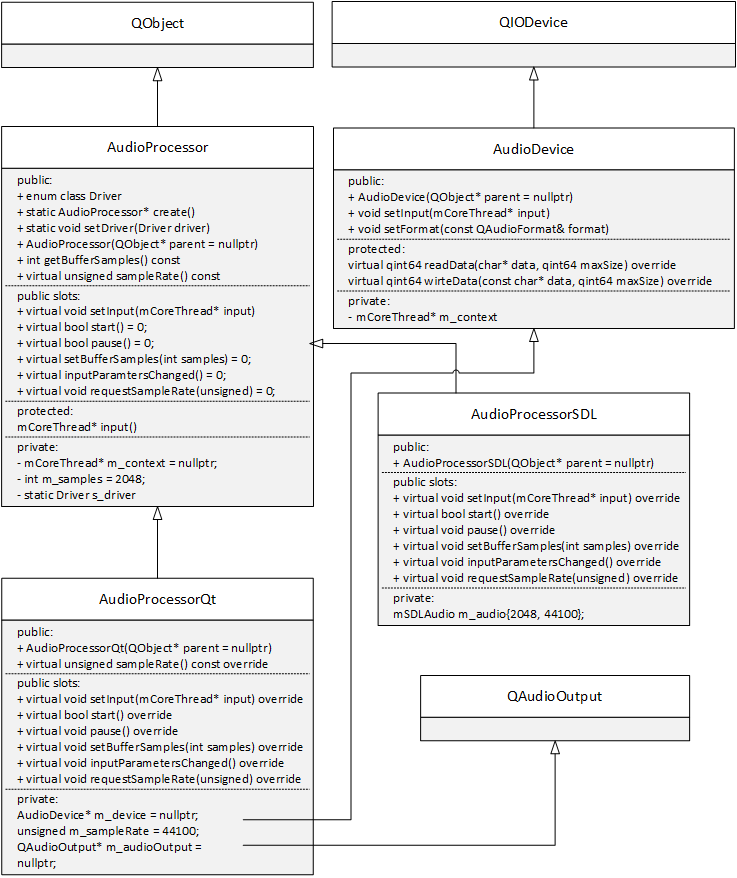
\includegraphics[width=0.7\textwidth]{QT_Klassendiagramm}
    \caption{Audioklassen in der QT-Anwendung}
    \label{fig:qtclassdiagramm}
\end{figure}

\newpage

\vspace{5mm}
\large AudioProcessor-Klasse \normalsize(\textit{\$/src/platform/qt/AudioProcessor.cpp})
\vspace{2mm}\newline
Die Klasse AudioProcessor erbt von QObject, ist eine abstrakte Klasse und definiert ein Interface f\"ur die Klassen AudioProcessorQt und AudioProcessorSDL. QObject ist die Basisklasse aller Qt Objekte und im Bezug auf
die Objektmodellierung somit das Herzst\"uck von Qt. 

\textbf{AudiProcessor::getBufferSamples} liefert die Anzahl der, intern in der Variablen m\_samples gespeicherten, Samples zur\"uck. Diese wird initial auf den Wert 2048 gesetzt. m\_samples kann mit dem Aufruf von \textbf{AudiProcessor::setBufferSamples} ge\"andert werden. Es folgen abstrakte Methoden und Slots. Diese werden in der Klasse \textbf{AudioProcessorQt} \"uberschrieben.

Weiterhin beinhaltet die Klasse eine Variable m\_context. Diese stellt einen Zeiger auf den mCoreThread dar und kann mit der Methode \textbf{AudioProcessor::setInput(mCoreThread* input)} gesetzt werden. 

Unter Verwendung einer selbst kompilierten Version von mGBA, mit Log-Ausgaben, konnte nach dem Erstellen der AudioProcessorQt-Klasse festgestellt werden, dass 
die \textbf{AudioProcessorQt::inputParameterChanged} Methode f\"unfmal aufgerufen wird. Gefolgt von einem Aufruf der \textbf{AudioProcessorQt::requestSampleRate} und dreimal der \textbf{AudioProcessorQt::inputParameterChanged} Methode. Ein weiterer Aufruf der \textbf{AudioProcessorQt::requestSampleRate} Methode folgt. Interessant an dieser Stelle ist, dass jeder Aufruf der zuvor aufgef\"uhrten Methoden bereits bei der \"Uberpr\"ufung ob ein \textbf{AudioDevice} vorhanden ist, scheitert. 
Daraus folgt, dass an dieser Stelle keine \"Anderungen vorgenommen werden. %Eine genauere Betrachtung der aufger\"uhrten Methoden folgt im folgenden Kapitel.

\subsubsection{Einstellungen \"uber die mGBA GUI} \label{kapitelEinstellungenMGBA}
\AutorFlorian

Der mGBA ist gestartet und die\textbf{AudioProcessorQt} wurde erstellt. Der Benutzer kann nun \"uber die Men\"uleiste Werkzeuge$\rightarrow$Einstellungen$\rightarrow$Audio/Video auf die Audio und Video Einstellungen zugreifen.

\begin{figure}[h!]
    \centering
    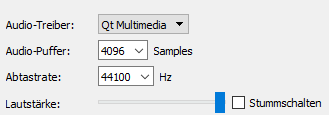
\includegraphics[width=0.7\textwidth]{Audioeinstellungen}
    \caption{Audioeinstellungen im mGBA}
    \label{fig:audioeinstellungen}
\end{figure}

In Abbildung \ref{fig:audioeinstellungen} sind die f\"ur dem Benutzer m\"oglichen Einstellungen im Bezug auf das Audiosystem dargestellt. Der Audio-Treiber kann entweder auf Qt Multimedia oder SDL eingestellt werden.
Der Audio-Puffer bietet die g\"angisten Anzahl an Samples von 512 bis 4096. Kann aber auch benutzerspezifische eingestellt werden. Weiterhin kann die Abtastrate gesetzt werden. Auch hier sind die g\"angigsten Raten vorgeschlagen, k\"onnen
aber auch frei gesetzt werden. Schlie{ss}lich folgt die Lautst\"arkeneinstellung.

Wie schon zu erahnen ist, wird nach einer Ver\"anderung des Audio-Treibers der Destruktor der zuvor gew\"ahlten Klasse aufgerufen und ein erneuter Aufruf der \textbf{AudioProcessor::create} Methode erzeugt eine neue AudioProcessor Instanz.
Anlie{\ss}end wird die Methode \textbf{AudioProcessor::setBufferSamples} aufgerufen. Als \"Ubergabeparameter erh\"ahlt diese den Wert aus dem Feld Audio-Puffer und setzt diesen in die interne Variable m\_samples.


\subsubsection{Starten des ROM}
\AutorFlorian

W\"ahlt der Benutzer eine neue ROM aus und startet diese, wird zun\"achst die \textbf{AudioProcessor::setInput} Methode aufgerufen. Diese setzt den Zeiger auf den m\_coreThread zur internen Variablen m\_context. Es folgt der Aufruf der
\textbf{AudioProcessorQt::start} Methode.

\vspace{5mm}
\large AudioProcessorQt::start() \normalsize(\textit{\$/src/platform/qt/AudioProcessorQt.cpp})
\vspace{2mm}\newline
Im ersten Schritt wird \"uberpr\"uft, ob der m\_coreThread bereits gesetzt wurde. Im n\"achsten Schritt wird der internen Variablen \textbf{m\_device} ein neue Instanz von \textbf{AudioDevice} zugewiesen.

Die Klasse \textbf{AudioDevice} stellt das Bindeglied zwischen AudioProcessorQt und dem mCoreThread dar. \textbf{AudioDevice} erbt von QIODevice. QIODevice ist ein Interface f\"ur alle I/O Ger\"ate und kann deshalb nicht direkt instanziiert werden.
Wird von dieser Basisklasse abgeleitet, m\"ussen die Methoden \textbf{readData} und \textbf{writeData} \"uberschrieben werden. Zus\"atzlich muss die Methode \textbf{setOpenMode} mit dem gew\"unschten Modus im Konstruktor aufgerufen werden. In diesem Fall wird der Parameter \enquote{ReadOnly} \"ubergeben. Daraus resultiert ein nur lesbares QIODevice. Weiterhin wird auch hier der mCoreThread \"ubergeben und gesetzt. Die bereits erw\"ahnte Methode \textbf{writeData} spielt hier keine Rolle, da nicht auf das Ger\"at geschrieben werden darf. Sie muss jedoch \"uberschrieben werden aber beinhaltet nur eine Warnung. Eine genauere Betrachtung der Funktionsweise der Klasse folgt.

Es folgt das Erzeugen einer neuen Instanz von QAudioFormat. Die Klasse \textbf{QAudioFormat} speichert Informationen \"uber Audio-Stream Parameter.

\vspace{5mm}
\begin{lstlisting}[language=C++, caption={Ausschnitt aus AudioProcessorQt::start()}, label={list:FormatAudioProcessorQt}]
    QAudioFormat format;
		format.setSampleRate(m_sampleRate); // m_sampleRate = 44100
		format.setChannelCount(2);			// 2 bedeutet Stereo 1 Mono
		format.setSampleSize(16);			// Typischerweise 8 oder 16
		format.setCodec("audio/pcm");		// Linear PCM
		format.setByteOrder(QAudioFormat::Endian(QSysInfo::ByteOrder));
		// Little- oder Big-Endian
		format.setSampleType(QAudioFormat::SignedInt);	// Sample Typ
		m_audioOutput = new QAudioOutput(format, this);
		m_audioOutput->setCategory("game");
\end{lstlisting}
  
Wie bereits am Ende von Snippet \ref{list:FormatAudioProcessorQt} zu sehen, wird eine neue Instanz der Klasse \textbf{QAudioOutput} erzeugt und in die interne Variable \textbf{m\_audioOutput} geschrieben. 
Dem Konstruktor der Klasse \textbf{QAudioOutput} wird das zuvor erstellte Format \"ubergeben.

\textbf{QAudioOutput} stellt ein Interface zur Verf\"ugung mit dem Audiodaten zu einem Audio-Ger\"at
gesendet werden k\"onnen(z.B. Lautsprecher, Kopfh\"orher usw.) Die \textbf{setCatecory} Methode setzt den Modus auf \enquote{game}. Einige Plattfomren k\"onnen Audio-Streams in Kategorien gruppieren.
N\"utzlich ist dieser Methodenaufruf, da unter Windows der mGBA nun im Lautst\"arken Mixer angezeigt wird.

Durch den Methodenaufruf \textbf{m\_device$\rightarrow$setInput} wird der Klasse \textbf{AudioDevice} der \textbf{mCoreThread} \"ubergeben. Daraufhin wird die \textbf{m\_device$\rightarrow$setFormat} Methode, mit einer Referenz auf
das Format von \textbf{m\_audioOutput} als \"Ubergabeparameter, aufgerufen.

\newpage

\vspace{5mm}
\large AudioDevice::setFormat(const QAudioFormat\& format) \normalsize(\textit{\$/src/platform/qt/AudioDevice.cpp})
\vspace{2mm}\newline 
Wie gewohnt wird zun\"achst \"uberpr\"uft, ob der \textbf{mCoreThread} vorhanden ist. Im n\"achsten Schritt wird ein Multiplikator errechnet. Dieser wird abh\"angig von der eingestellten FPS berechnet. Bei 60 FPS betr\"agt dieser
0,995458. Anschli{\ss}end werden die im \textbf{mCoreThread} befindlichen Audio-Speicherbereiche gesperrt. Nun werden die Frequenzen der beiden Audiokan\"ale im \textbf{mCoreThread} mit den Frequenzen, multipliziert mit dem zuvor errechneten
Multiplikator, des \textbf{m\_audioOutput} synchronisiert. Mit dem entsperren der Speicherbereiche endet die Methode.

Zur\"uck in der \textbf{AudioProcessorQt::start} Methode wird mit dem Aufruf von \textbf{m\_audioOutput$\rightarrow$start(m\_device)} die Audioausgabe gestartet. Schlie{\ss}lich wird der Status des \textbf{m\_audioOutput} auf aktive gesetzt.
Konnte der Status erfolgreich auf aktiv gesetzt werden, liefert \textbf{AudioProcessorQt::start} \enquote{true} zur\"uck.
 
\subsubsection{Transferirrung der Audiodaten}
\AutorFlorian

Wie bereits im vorangegangenen Kapitel erw\"ahnt, wird der \textbf{m\_audioOutput$\rightarrow$start} Methode das \textbf{AudioDevice} \"ubergeben. Dies bewirkt, dass die Klasse \textbf{QAudioOutput} jetzt von der Klasse \textbf{AudioDevice} 
Daten f\"ur die Audioausgabe liest und diese an die Systemausgabe weiterleitet. Einmal gestartet, l\"auft die Audioausgabe kontinuierlich weiter. Nur ein Aufruf der Methode \textbf{AudioProcessorQt::pause} stoppt die Ausgabe.

Die Klasse \textbf{QAudioOutput} ruft nun selbstst\"andig  in gewissen Zeitabst\"anden die \textbf{AudioDevice::readData} Methode auf und \"ubergibt einen Zeiger in dem die Daten zur Ausgabe eingelesen werden sollen und dessen Gr\"o{\ss}e.

\vspace{5mm}
\large AudioDevice::readData(char* data, qint64 maxSize) \normalsize(\textit{\$/src/platform/qt/AudioDevice.cpp})
\vspace{2mm}\newline
Wie bereits erw\"ahnt, muss diese Methode \"uberschrieben werden. Zu Beginn wird \"uberpr\"uft ob die maximal zul\"assige Gr\"o{\ss}e des \"ubergebenen Puffers nicht \"uberschritten ist und der \textbf{m\_coreThread} vorhanden ist.
Nun wird, wie auch in der \textbf{AudioDevice::setFormat} Methode, der Speicherbereich im \textbf{m\_coreThread} in dem die Audiodaten gespeichert sind gesperrt.
Mit dem Methodenaufruf \textbf{blip\_samples\_avail} wird die Anzahl der verf\"ugbahren Samples im \textbf{m\_coreThread} abgefragt. \"Uberschreitet die Anzahl der Samples die Gr\"o{\ss}e des Puffers, geteilt durch die 
Strukturgr\"o{\ss}e \textbf{GBAStereoSample}, wird die Anzahl der verf\"ugbahren Samples auf die Puffergr\"o{\ss}e, geteilt durch die Strukturgr\"o{\ss}e \textbf{GBAStereoSample}, reduziert.

Jetzt k\"onnen die Samples aus dem \textbf{m\_coreThread} gelesen werden. Dies geschieht durch den Methodenaufruf von \textbf{blip\_read\_samples} f\"ur den linken und den rechten Kanal. 
Dazu wird der \"ubergebene Puffer auf die Struktur \textbf{GBAStereoSample} gecastet und \"ubergeben. Ein Entsperren des zuvor gesperrten Speicherbereichs und das Zur\"uckgeben der Anzahl gelesener Daten beendet die Methode
\textbf{AudioDevice::readData}. Die im Puffer befindlichen Daten werden nun in der Klasse \textbf{QAudioOutput} verarbeitet und zum Systemausgang weitergeleitet.


\newpage

% ========== Chapter 4 ==========

\section{Zusammenfassung} \label{Zusammenfassung}

% ========== Chapter 4.1 ==========

\subsection{Inhalt des Dokumentes}
\AutorDominik

% ========== Chapter 4.2 ==========
\subsection{Fazit zur Studienarbeit}

\large Dominik Scharnagl
\vspace{2mm}\newline
Hello World by Dominik.

\vspace{5mm}
\large Florian Boemmel
\vspace{2mm}\newline
Hello World by Florian.

\vspace{5mm}
\large Ngoc Luu Tran
\vspace{2mm}\newline
Hello World by Ngoc.


\newpage
\addtocontents{toc}{\protect\setcounter{tocdepth}{-1}}

\begin{thebibliography}{tiefe}
    \bibitem{NintendoGeschichte}Nintendo: \textit{Game Boy Advance}\newline
    \url{https://www.nintendo.de/Unternehmen/Unternehmensgeschichte/Game-Boy-Advance/Game-Boy-Advance-627139.html}, Mai 2018
    \bibitem{GigaEmulator}Giga Ratgeber: \textit{Was ist der Unterschied zwischen Simulation, Emulation \& Virtualisierung?}\newline
    \url{https://www.giga.de/extra/ratgeber/specials/was-ist-der-unterschied-zwischen-simulation-emulation-virtualisierung-computertechnik/}, Mai 2018
    \bibitem{GameBoyTechnischeDaten}Nintendo: \textit{Game Boy Advance}\newline
    \url{http://de.nintendo.wikia.com/wiki/Game_Boy_Advance}, Mai 2018
    \bibitem{GameBoySoundsystem}Coranac: \textit{18. Beep! GBA sound introduction}\newline
    \url{https://www.coranac.com/tonc/text/sndsqr.htm#sec-intro}, Mai 2018
    \bibitem{SoundRegisters}BELOGIC: \textit{The Audio ADVANCE}\newline
    \url{http://belogic.com/gba/}, Juni 2018
\end{thebibliography}

\vspace{1cm}

\huge Bilder
\normalsize

\begin{itemize}
    \item Abbildung \ref{fig:gba}: \textit{Game Boy Advance - Blue Edition}\newline
    \url{https://d3nevzfk7ii3be.cloudfront.net/igi/L3WryntCMswfDks1.large}, Mai 2018
\end{itemize}

\begin{itemize}
    \item Abbildung \ref{fig:qtclassdiagramm}: \textit{\"Ubersicht der Audioklassen in der Qt Anwendung}
\end{itemize}

\end{document}











